\chapter{Background and Related Work}
\label{chap:background}
This chapter establishes the theoretical foundations and reviews related work necessary for the proposed system. It starts by introducing the Robot-in-the-Loop testing paradigm in Section~\ref{sec:RitL}. Section~\ref{sec:DT} provides an overview of Digital Twin technology, followed by a discussion on Mixed Reality in Section~\ref{sec:MR}. The Robot Operating System 2, which serves as the communication backbone, is described in Section~\ref{sec:ros2}. Section~\ref{sec:vera} details the VERA framework that this work builds upon and highlights its current limitations. To address these, Section~\ref{sec:sim_engines} evaluates suitable simulation engines. Finally, Section~\ref{sec:synthesis_objectives} synthesizes the findings to outline the objectives of this thesis.
 \section{Robot-in-the-Loop-Testing}
\label{sec:RitL}
The validation and verification of modern Robotic and Autonomous Systems (RAS) is a significant challenge due to their complexity~\cite{AMV23}. This is because they integrate software, mechanical, and electrical engineering all at once~\cite{AMV23}. A central problem is ensuring that the software and hardware work together seamlessly, especially when testing both simultaneously~\cite{AMV23}. The X-in-the-Loop (XitL) simulation paradigm addresses this challenge~\cite{Brayanov2019}. It provides a framework to integrate the flexibility of software simulation with the realism of physical experiments~\cite{Brayanov2019}.

A foundational XitL method is Hardware-in-the-Loop (HitL) simulation, which is a technique for testing mechatronic systems~\cite{Mihalic2022, Brayanov2019}. The main principle of HitL is creating a closed loop between the real hardware that is being tested and a simulation that represents the rest of the system or its operational environment~\cite{Mihalic2022}. This setup effectively simulates the hardware to respond as if it were operating in a real system, which allows for testing across a wide range of virtual scenarios~\cite{Brayanov2019}. The main reason for using HitL is to shorten development cycles and prevent costly or dangerous failures by making exhaustive testing possible before the system is completely implemented~\cite{Mihalic2022}. This is why HitL is essential in industries like automotive, aerospace, and robotics, where real-world testing can be too expensive, dangerous, or even impossible~\cite{Brayanov2019}.

Robot-in-the-Loop (RitL)~\cite{Mihalic2022} simulation extends the HitL concept. Instead of just a component, the hardware under test is a complete robotic system, such as an uncrewed vehicle~\cite{Mihalic2022}. RitL replaces components of a pure simulated setup with the actual robot, increasing the realism of testing~\cite{Hu05}. A typical RitL configuration has the robot's real actuators operating in the physical world, while its sensors interact with a simulated environment instead~\cite{Hu05, Mihalic2022}. This creates a hybrid setup where, for example, the robot might use virtual sensors to see objects in the simulation but use its real motors to move physically~\cite{Hu05}. To keep the physical and virtual worlds synchronized, the real robot often has a virtual counterpart in the simulation whose state is updated as the physical robot acts and moves~\cite{Hu05}.



The main benefit of RitL is that it uses the dynamics of actual hardware for repeatable testing of high-level software, such as navigation algorithms~\cite{Mihalic2022}. This method avoids the expense, complexity, and risk of full physical testbeds while being a secure and useful substitute~\cite{Mihalic2022}. RitL therefore becomes a tool for safely evaluating system performance in the lab~\cite{Hu05, Mihalic2022}. This is especially important when working on projects that are hard to replicate, such as large-scale robot swarms or Mars rover missions, or when safety is at risk~\cite{Hu05, Mihalic2022}.

The RitL paradigm has been widely applied to validate complex autonomous systems, particularly in the automotive field using Vehicle-in-the-Loop (VitL) testing. For example, the Dynamic Vehicle-in-the-Loop (DynVitL) architecture integrates a real test vehicle with the high-fidelity CARLA simulator, which operates on the Unreal Engine~\cite{DSR22}. As shown in Figure~\ref{fig:vitl_setup}, this approach allows a vehicle on an empty track to be stimulated by sensor data from a virtual world~\cite{DSR22}. This allows automated driving functions to be safely and reliably tested in situations that would be hazardous to physically replicate~\cite{DSR22}. CARLA and the Unreal Engine are also used in a similar Vehicle-in-Virtual-Environment (VVE) method which establishes a closed loop in which the motion of the real vehicle is tracked and reflected in the virtual world, making it possible for its control systems to respond to simulated events~\cite{Cao2023}.

\begin{figure}[H]
\centering
\includegraphics[width=0.9\textwidth]{images/vehicle_in_the_loop_dsr+22.jpg}
\caption{An example of a VitL setup. A real car on a test track connected to a high-fidelity simulator like CARLA that generates virtual traffic and sensor data.~\cite{DSR22}}
\label{fig:vitl_setup}
\end{figure}

These examples show a trend towards using game engine based simulators to evaluate autonomous vehicles. This method falls somewhere between physical testing, where safety and consistency can be problematic, and pure software simulation, which frequently lacks vehicle dynamics fidelity~\cite{Cao2023}. Some systems even stimulate the vehicle's actual sensors. For instance, the Radar Target Simulator (RTS) can feed artificial radar echoes from a virtual scene to the vehicle's actual radar sensor~\cite{Diewald2021}. This allows for end-to-end validation of the entire perception and control pipeline~\cite{Diewald2021}.

The X-in-the-Loop approach is found in many different areas. In marine robotics, a VitL framework was developed to test the long-term autonomy of a robot swarm. In this system, an Autonomous Surface Vehicle (ASV) interacts with multiple simulated underwater sensor nodes to test cooperative behaviors without the logistical cost of deploying a full swarm~\cite{Babic2020}. In the aerospace domain, the RFlySim platform uses a Field Programmable Gate Array (FPGA)-based HitL system to create a high-fidelity simulation for testing Unmanned Aerial Vehicle (UAV) autopilot systems in a lab, which reduces the need for expensive and risky outdoor flights~\cite{Dai2021}.

These approaches continue to move toward deeper integration. The Scenario-in-the-Loop (SciL) paradigm creates a mixed reality that blurs the boundary between physical testing and virtual simulation~\cite{Varga2021}. Unlike standard HitL methods, SciL allows the simulation to actively drive the physical environment~\cite{Horvath2019}. A central software system uses virtual triggers to physically actuate real-world infrastructure, such as moving robotic dummies or changing traffic signals~\cite{Horvath2019}. Simultaneously, the system manipulates the vehicle's perception using Augmented Reality (AR) to inject synthetic data directly into the vehicle's communication network alongside physical sensor readings~\cite{Varga2021}. As a result, the vehicle cannot distinguish between physical objects and virtual ones~\cite{Varga2021}. This indistinguishable perception compels the vehicle to execute real control maneuvers, such as emergency braking, in response to purely digital stimuli~\cite{Varga2021}.

\section{Digital Twins}
\label{sec:DT}
The Digital Twin is an important concept in many current X-in-the-Loop frameworks. The Digital Twin serves as the virtual counterpart to a physical system, acting as a virtual copy that allows real-time monitoring and simulation~\cite{AA23}. The idea is to create a digital information model of a physical system that stays linked to it for the duration of its lifecycle~\cite{Grieves2017}.

This concept was initially known as the Information Mirroring Model and consists of three core elements: the physical product, its corresponding virtual model, and the data connection that connects them~\cite{Grieves2017, AA23}. A diagram of this structure is shown in Figure~\ref{fig:dt_concept}. The virtual model extends beyond a representation of physical dimensions; it is often a detailed simulation that can model mechanical, electrical, and software properties of a system~\cite{Leng2021}. Information moves in both directions, so sensor data can flow from the real world to update the virtual model~\cite{Grieves2017, Leng2021}. In turn, the virtual model can also send commands back to control or optimize the physical system~\cite{Grieves2017, Leng2021}. This continuous, bidirectional data exchange characterizes a Digital Twin~\cite{AA23}.

\begin{figure}[H]
\centering
\includegraphics[width=0.8\textwidth]{images/info_mirror_model_Grieves15.png}
\caption{The foundational concept of a Digital Twin, illustrating the three core components: the physical entity, the virtual model and the bi-directional data connection that links them~\cite{Grieves2017, Leng2021}.~\cite{Grieves15}}
\label{fig:dt_concept}
\end{figure}

Digital Twins in robotics are frequently created using simulation software and the middleware that connects the virtual simulation to the actual hardware is often the Robot Operating System (ROS)~\cite{MFG22}. Stączek et al. used the Gazebo simulator with ROS to create a digital twin of a factory floor, which they used to test and optimize the navigation algorithms of a mobile robot in narrow corridors~\cite{Staczek2021}. To validate a deep learning-based harvesting robot, R. Singh et al. adopted a similar strategy and created a digital twin of a greenhouse in Gazebo~\cite{Singh2024a}. Other simulators like CoppeliaSim and Webots are also common. Magrin et al. used CoppeliaSim and ROS to create a digital twin as a learning tool for mobile robot design~\cite{Magrin2021}, while Marques et al. used Webots for an Automated Guided Vehicle (AGV), synchronizing it via an OPC-UA server~\cite{Marques2024}. These examples show a common approach of using simulators to simulate robot kinematics and sensor feedback for closed-loop testing.
 
More recently, game engines have become a popular choice for creating Digital Twins, as they offer more realistic graphics and physics. Unity~\cite{Uni23}, for instance, is used to build highly realistic virtual environments. Pérez et al. utilized Unity to develop a digital twin of a robotic cell, which is a manufacturing station where robots, conveyors, and safety systems work together to perform tasks~\cite{Perez2020}. In this framework, the digital twin acts as a live mirror of the physical cell~\cite{Perez2020}. The system uses the game engine to simulate physical laws and mechanical behaviors, ensuring that the virtual robots act exactly like the real ones~\cite{Perez2020}. To achieve this synchronization, the virtual model connects directly to the facility's control network to read real-time data from the sensors~\cite{Perez2020}. This connectivity allows engineers to virtually validate the cell's design and logic before any equipment is installed and subsequently enables operators to train safely alongside the virtual robots~\cite{Perez2020}.

Another important consideration is the technical capabilities of these engines. Yang et al.~\cite{Yang2020} simulated the physics of a UAV using Unity and its built-in NVIDIA PhysX engine. They also demonstrated the creation of virtual sensors, such as a Light Detection and Ranging (LiDAR) sensor, directly within the game engine using its raycasting Application Programming Interface (API)~\cite{Yang2020}. Research has also been done on the performance and reliability of these game engine-based frameworks. Kwon et al. developed a safety-critical Digital Twin integrated with Unity and ROS 2, which achieves minimal data transmission latency to enable the prediction of collisions in real time~\cite{Kwon2025}. 

\section{Mixed Reality}
\label{sec:MR}
Beyond the testing paradigm and the digital twin, the way a user interacts with the system is another part of a robotics framework. Virtual, Augmented, and Mixed Reality have become promising technologies for improving the information exchange between humans and robots~\cite{Walker2023}. In robotics, Augmented Reality (AR) is an especially useful tool for enhancing Human-Robot Interaction (HRI) by integrating virtual objects into a real-world environment in real time~\cite{MV20}.

The relationship between these technologies is formally described by the foundational Reality-Virtuality Continuum concept, first introduced by Milgram and Kishino~\cite{MK94}. As illustrated in Figure~\ref{fig:rv_continuum}, this continuum is a scale that is anchored by a purely real environment at one end and a completely virtual one at the other~\cite{MK94, Skarbez2021, MV20}.

\begin{figure}[H]
\centering
\includegraphics[width=0.9\textwidth]{images/reality_virtuality_continuum_wpc+23.png}
\caption{The Reality-Virtuality Continuum, illustrating the spectrum from a real environment to a completely virtual one.~\cite{Walker2023}}
\label{fig:rv_continuum}
\end{figure}

A Virtual Reality (VR) environment is an endpoint of the continuum, where the user is totally immersed in and can interact with a fully synthetic world~\cite{MK94}. This approach is useful for HRI research, as it allows for testing interactions with virtual robots in scenarios where it might be unsafe or too expensive for physical hardware~\cite{Walker2023}. The general term Mixed Reality (MR) describes the entire spectrum between the two extremes, where real and virtual worlds are combined into a single display~\cite{MK94}. MR is made up of two main categories: AR and Augmented Virtuality (AV)~\cite{MK94, MV20}. AR is the process of adding virtual objects to a real environment~\cite{MK94}. This allows, for example, HRI researchers to place 3D data and intentions of a robot directly into the physical space of a user~\cite{Walker2023}. The opposite is Augmented Virtuality (AV), where a primarily virtual world is enhanced with elements from the real world, like live video feeds~\cite{MK94}.

\section{Robot Operating System 2}
\label{sec:ros2}
Robot Operating System 2 (ROS~2) is not an operating system but a middleware framework to simplify the creation of complex robotic systems~\cite{MFG22}. It was redesigned from scratch to meet the challenges posed by modern robotics in domains ranging from logistics and agriculture to space missions and became the standard for both research and industry~\cite{macenski2023survey, MFG22}. At its core, ROS~2 is designed based on principles of distribution, abstraction, asynchrony, and modularity that together allow the development of scalable and robust applications~\cite{MFG22}.
The architecture of ROS~2 is based on a distributed network of independent programs called Nodes~\cite{MFG22}. A node is a single, self-contained executable that performs a specific task, such as controlling a motor, processing sensor data, or, in the case of this thesis, bridging communication between robots and the simulation~\cite{MFG22}. The nodes communicate through a set of defined patterns. The most common pattern is the publish-subscribe mechanism called Topics, illustrated in Figure~\ref{fig:ros2_comm_concept}~\cite{MFG22}. In this model, nodes can publish data as messages to a topic, while other nodes can subscribe to that topic to receive data asynchronously~\cite{MFG22}. For tasks that require a direct request and a guaranteed response, ROS~2 offers Services, following a synchronous request-response pattern~\cite{MFG22}. For long-running tasks that require continuous feedback and the ability to be preempted, ROS~2 provides a unique communication pattern called Actions~\cite{MFG22}. An action consists of a goal, a feedback stream, and a final result, making it optimal for managing tasks like navigation where the progress of a robot toward a goal has to be monitored over time~\cite{macenski2020marathon2}.

\begin{figure}[H]
    \centering
    \begin{tikzpicture}[node distance=1.5cm and 2cm, auto, >=stealth]
        % --- NODES USING THE 'align' OPTION FOR ROBUSTNESS ---
        \node[draw, rectangle, rounded corners, align=center] (pub_node) {Node A \\ \textbf{(Publisher)}};
        \node[draw, ellipse, fill=blue!20, right=of pub_node, align=center] (topic) {Topic \\ \texttt{/sensor\_data}};
        \node[draw, rectangle, rounded corners, right=of topic, align=center] (sub_node1) {Node B \\ \textbf{(Subscriber)}};
        \node[draw, rectangle, rounded corners, below=of sub_node1, yshift=-0.25cm, align=center] (sub_node2) {Node C \\ \textbf{(Subscriber)}};

        % Arrows
        \draw[->, thick] (pub_node) -- (topic) node[midway, above] {Message};
        \draw[->, thick] (topic) -- (sub_node1);
        \draw[->, thick] (topic) -- (sub_node2);
    \end{tikzpicture}
    \caption{The ROS~2 publish-subscribe model. Node A publishes messages onto a central topic and any number of subscriber nodes (B and C) may receive that data without direct knowledge of the publisher.}
    \label{fig:ros2_comm_concept}
\end{figure}

An essential part of any mobile robot is coordinate frame management, which in ROS~2 is accomplished through its transform library, tf2~\cite{foote2013tf}. The tf2 library standardizes the tracking of spatial relationships between the various parts of the robot and environment, placing them into a tree-like data structure, as illustrated in Figure~\ref{fig:tf_tree_concept}~\cite{foote2013tf}. This permits any node in the system to request at any time the position and orientation of any frame relative to another, a feature critical for transforming sensor data into a useful frame of reference~\cite{foote2013tf}.

\begin{figure}[H]
    \centering
    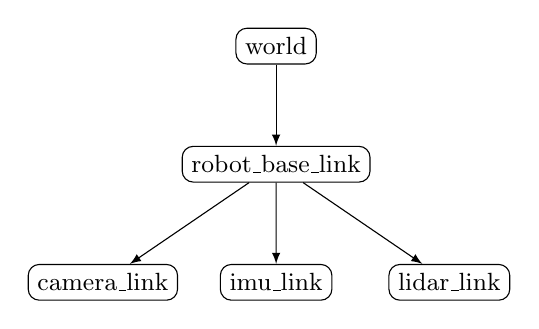
\begin{tikzpicture}[
        level 1/.style={sibling distance=3.5cm},
        level 2/.style={sibling distance=2.2cm}, % Adjusted spacing
        edge from parent/.style={draw, -latex},
        every node/.style={draw, rectangle, rounded corners, text centered, font=\small} % Made font slightly smaller for compactness
    ]
    \node {world}
        child { node {robot\_base\_link}
            child { node {camera\_link} }
            child { node {imu\_link} }
            child { node {lidar\_link} }
        };
    \end{tikzpicture}
    \caption{A simplified example of a ROS~2 transform tree (tf tree). The library maintains the hierarchical relationships so that a program can easily determine the transform from the \texttt{camera\_link} to the \texttt{world} frame, for instance.}
    \label{fig:tf_tree_concept}
\end{figure}

In the architecture of this thesis, ROS~2 provides the central data backbone, a term borrowed from digital engineering that defines an integrated communication layer for all relevant system knowledge~\cite{perzylo2020backbone}. This acts as the bridge that couples the physical EMAROs robot and its tracking system with the simulation environment. The digital twin of the EMAROs robot subscribes to ROS~2 topics to receive real-time data from the physical world and can synchronize its state through this communication layer~\cite{singh2024unity}.
For navigation of both the physical and virtual robots, this thesis utilizes Navigation2 (Nav2), the official, next-generation autonomous navigation framework for ROS~2 ~\cite{macenski2020marathon2}. Nav2 was designed from the ground up to orchestrate planning, control and recovery tasks using configurable Behavior Trees that are highly modular and can be changed at runtime to create custom navigation behaviors ~\cite{macenski2020marathon2}. Core to its operation, Nav2 separates the navigation task into two closely related, yet distinct components, namely a global planner, which seeks out an acceptable, long-range path through the environment and a local trajectory planner or controller, which generates velocity commands in order to follow that route while reacting to immediate obstacles ~\cite{macenski2023survey}. Using the Nav2 stack, a high-level goal, e.g., a coordinate in the environment, can be sent via a ROS~2 action to a robot and the system will take care of all complex path planning and collision avoidance autonomously.
\section{The VERA Framework}
\label{sec:vera}

This thesis directly builds on the Virtual Environment for mobile Robotic Applications framework, which was developed earlier by Gehricke~\cite{Geh24}. VERA was designed initially as a modular and scalable platform to bridge the validation gap between pure software simulation and real-world testing. It combines the concepts of Digital Twins, AR and Vehicle-in-the-Loop testing to enable robots to interact with a virtual environment projected into the real world~\cite{Geh24}.

The core idea of VERA is projecting a dynamic, interactive virtual world onto the physical floor where a real robot operates. The system synchronizes the virtual state with the actions of the physical robot in such a way that scenarios are possible where the robot can detect and react to virtual obstacles as if they were real. This system provides a flexible testbed for the development and evaluation of robotic applications without having to physically build complex environments~\cite{Geh24}.

\begin{figure}[H]
    \centering
    \includegraphics[width=0.8\textwidth]{images/vera_setup.jpg}
    \caption{The physical setup of the VERA platform: A projector and tracking system are mounted on a frame above the test area.~\cite{Geh24}}
    \label{fig:vera_setup}
\end{figure}

\subsection{EMAROs Test Platform}
\label{sec:EMAROs_platform}
The capabilities of VERA are demonstrated by a mobile mini-robot called the Educational Modular Autonomous Robot Osnabrück (EMAROs), shown in Figure~\ref{fig:EMAROs_robot}, which was developed at Osnabrück University specifically for research and education in robotics and artificial intelligence~\cite{EMAROs_Ref}.
The modular hardware architecture of EMAROs is based on three main PCBs: a Host PCB containing high-level computing, a Power PCB managing energy supply and motor control, and a Base PCB integrating ground sensors~\cite{Geh24}. The specific variant used in this work is equipped with a Raspberry Pi Compute Module 4 (CM4) running Ubuntu~24.04 and ROS~2~\cite{Geh24}.

\begin{figure}[H]
    \centering
    \includegraphics[width=0.5\textwidth]{images/EMAROs_robot.png}
    \caption{The EMAROs robot is the robotic platform used in the testbed, equipped with a modular sensor suite and running ROS~2.~\cite{Geh24}}
    \label{fig:EMAROs_robot}
\end{figure}

For obstacle avoidance, the robot is equipped with Time-of-Flight (ToF) distance sensors and an Inertial Measurement Unit (IMU) for orientation tracking~\cite{Geh24}. Moreover, there are two wide-angle cameras that can be configured for stereo vision applications or line-following tasks~\cite{Geh24}. Within VERA, EMAROs takes on the role of the robot, streaming real-time telemetry including odometry, battery status, and sensor data to the simulation framework via ROS~2 to create a digital twin~\cite{Geh24}.

\subsection{Original VERA System Architecture}
The software architecture of the original VERA framework was mainly a ROS~2 implementation and its structure included only three main components: the Virtual Environment Positioning System (VEPS), the Environment Manager and the Visualization System~\cite{Geh24}.

Accurate localization is important to synchronize the physical robot with the projected virtual world and was provided by the VEPS in the original VERA framework~\cite{Geh24}. The original VEPS implementation relied on a depth-based approach where a ceiling-mounted Allied Vision Ruby 3D stereo camera captured point clouds of the test area~\cite{Geh24}. The point clouds were filtered by a Median Absolute Deviation (MAD) algorithm to calculate the centroid of the robot~\cite{Geh24}.
However, for maximum robustness and precision for this thesis, the positioning system was updated to use an ArUco marker-based tracking system developed in parallel research by~\cite{JuliaBA}, as shown in Figure~\ref{fig:veps_comparison}. Although the point-cloud method provided a markerless solution, the ArUco-based approach has higher reliability and lower noise~\cite{JuliaBA,Geh24}. By attaching a fiducial marker to the top of the EMAROs robot, the system is able to calculate the 6D pose (position and orientation) of the robot~\cite{JuliaBA}. This pose is published into the ROS~2 network, where it can instantly update the position of the digital twin~\cite{JuliaBA}.


\begin{figure}[H]
    \centering
    % Linkes Bild (nimmt 49% der Textbreite ein)
    \begin{minipage}{0.64\textwidth}
        \centering
        \includegraphics[width=\linewidth]{images/point_cloud.png}
    \end{minipage}%
    \hfill% Abstandhalter
    % Rechtes Bild (nimmt 49% der Textbreite ein)
    \begin{minipage}{0.36\textwidth}
        \centering
        \includegraphics[width=\linewidth]{images/arcuo.jpg}
    \end{minipage}
    \caption{The original VERA used point clouds~\cite{Geh24}, while the current iteration uses ArUco markers for pose estimation~\cite{JuliaBA}.}
\end{figure}
The \textbf{Virtual Environment Manager} is the central brain of the simulation~\cite{Geh24}. Implemented as a C++ ROS~2 node, it parses environment definitions from standard Gazebo \texttt{world.sdf} files~\cite{Geh24}. It keeps track of the state of all virtual objects, including their positions and properties, such as whether an object is movable or static~\cite{Geh24}.
One of the key roles of the manager is to manage the interactions of the robot with the virtual world~\cite{Geh24}. It operates a continuous loop, typically at 20 Hz, which checks the distance between the position of the robot given by the VEPS and the virtual objects~\cite{Geh24}. The manager triggers predefined actions if a collision is detected, such as removing a manipulatable object or stopping the robot~\cite{Geh24}. It relies on basic distance heuristics and not a physics engine, hence limiting interactions to simple ones~\cite{Geh24}.

The \textbf{Visualization System} is responsible for rendering the virtual environment so it can be projected onto the physical floor~\cite{Geh24}. In the original VERA framework, this was achieved using a custom ROS~2 node and Pygame, a Python library designed for 2D game development~\cite{Geh24}.
The visualizer subscribes to the object lists published by the Manager and the robot's path history~\cite{Geh24}. It provides a 2D, top-down, orthogonal view of the scene, drawing obstacles as simple geometric shapes~\cite{Geh24}. It gives Augmented Reality features, projecting dynamic information directly into the workspace~\cite{Geh24}. The driven path of the robot is displayed as a trail, while a system status panel with real-time CPU and battery usage is shown behind the robot, as illustrated in Figure~\ref{fig:pygame_vis}~\cite{Geh24}.

\begin{figure}[H]
    \centering
    \includegraphics[width=0.8\textwidth]{images/pygame_visualizer.png}
    \caption{Original VERA visualization via Pygame, showing a projection of the robot's path and virtual obstacles onto the floor.~\cite{Geh24}}
    \label{fig:pygame_vis}
\end{figure}

\subsection{Identified Limitations}
\label{sec:vera_limitations}
While VERA successfully demonstrated the concept of Robot-in-the-Loop testing with AR projections, its original software implementation contains several critical limitations, that this thesis sets out to overcome:
\begin{itemize}
    \item \textbf{Lack of Realistic Physics:} The custom Environment Manager does not feature a physics engine~\cite{Geh24}. Collision detection is performed through simple radius checks, meaning the robot cannot push objects or experience friction nor can it interact with complex geometries~\cite{Geh24}. This reduces the realism of the digital twin~\cite{Geh24}.
    \item \textbf{Performance Scalability:} The Pygame-based visualizer utilizes the CPU for rendering and has performance-related issues for complex scenarios~\cite{Geh24}. Gehricke~\cite{Geh24} noted that in environments with a high number of dynamic objects (e.g., $>$800), the message queue became saturated, leading to considerable latency and incomplete visual updates.
    \item \textbf{Limited Interaction (No VR):} The system was designed strictly for 2D floor projections and Rviz~\cite{Geh24}. It does not support any kind of immersive VR interfaces that would enable a human operator to view the scene in 3D or to interact with the robot remotely~\cite{Geh24}. Therefore, the integration of VR was identified as a necessary future step for Human-Robot Interaction (HRI)~\cite{Geh24}.
\end{itemize}

\section{Simulation Engines for Robotics}
\label{sec:sim_engines}
The choice of a capable simulation engine is an important part in solving the limitations of the original VERA framework. The choice of platform affects the efficiency, accuracy, and applicability of the digital twin~\cite{Singh2025}. Based on this, the review of simulation engines in this thesis is guided by four criteria which are required for a functional MR digital twin:
\begin{itemize}
    \item \textbf{High Visual Fidelity:} Rather than focusing solely on graphical aesthetics, high visual fidelity is essential for generating accurate data for visual sensors (e.g., cameras) and ensuring user immersion in VR, addressing a significant limitation of robotics simulation platforms~\cite{dosSantos2025}.
    \item \textbf{Physics Accuracy:} To accurately predict the kinematic and dynamic behavior of the EMAROs robot, the engine needs to have a strong physics backend~\cite{Singh2025}.
    \item \textbf{Native VR/AR Support:} In order to extend VERA with the proposed Virtual Reality interfaces, the engine must have a framework for VR devices and provide capabilities for creating interactive environments without extensive middleware~\cite{Coronado2023}.
    \item \textbf{Robust ROS~2 Integration:} ROS~2 forms the data backbone~\cite{perzylo2020backbone} of the system and should enable low-latency, high-throughput communication to synchronize the digital twin with the physical robot in real time~\cite{Singh2025}.
\end{itemize}

\subsection{Robotics Simulators}
\textbf{Gazebo} is the most widely used simulator in Industry 4.0 applications because of its deep integration with ROS, and it is open-source~\cite{Singh2025}. It delivers detailed physics simulations along with sensor data emulations, making it ideal for precise engineering applications~\cite{Singh2025}. However, while this simulator benefits from a large community and extensive documentation, there are noticeable drawbacks concerning visualization~\cite{dosSantos2025}. For example, the rendering quality of Gazebo is only moderate and not photorealistic to an extent that would enable immersive VR experiences~\cite{dosSantos2025}. Moreover, some works note that Gazebo has a steep learning curve for new users due to its complex configuration and less intuitive user interface compared to modern commercial tools~\cite{Singh2025, Gonzalez2025}.

\textbf{Webots} is a well-established open-source platform, appreciated for cross-platform support and a large library of robot models~\cite{Kargar2024}. Although it is quite effective in educational applications, the rendering capabilities of the software are somewhat dated compared to the current game engines, making it not fitting for high-fidelity MR graphics~\cite{Kargar2024}.

\subsection{Physics-Based Simulators}
A few other simulators were found in literature but considered less appropriate for the particular VR needs of this thesis. CoppeliaSim (previously known as V-REP) is widely applied in automation, yet it has less physics realism compared to the professional ones and its scaling is limited~\cite{Gonzalez2025}. MuJoCo does well with contact-rich tasks and Reinforcement Learning but works almost exclusively on the stability of the physics and not the visualization, so it lacks the inbuilt VR frameworks necessary for MR interaction~\cite{Gonzalez2025}.

\subsection{High Visual Fidelity and Game-Based Engines}
Game engines have been widely adopted within the robotics community to overcome the visualization limitations of traditional robotics simulators.

\textbf{NVIDIA Isaac Sim} is the state-of-the-art in industrial simulation~\cite{dosSantos2025}. The platform is capable of photorealism through ray-tracing and has advanced GPU-accelerated physics through PhysX~\cite{dosSantos2025}. It excels in generating synthetic data for AI perception~\cite{Kargar2024}. But Isaac Sim has a very high hardware barrier where high-end NVIDIA RTX GPUs are specifically mandatory~\cite{dosSantos2025}. Being proprietary, it is more restricting for use in educational contexts compared to more open-source or widely accessible game engines~\cite{dosSantos2025}.

\textbf{Unreal Engine} is renowned for photorealistic visuals and is capable of handling big, open-world environments~\cite{Gonzalez2025}. But it has a steep learning curve because of its dependency on C++, and therefore is not very well-suited for rapid prototyping compared to other engines like Unity~\cite{Coronado2023}.

\textbf{Unity Engine} is establishing itself as the primary platform for Industry 5.0 applications, in particular those focusing on HRI and MR~\cite{Gonzalez2025}. It boasts a balance of high-fidelity graphics with a robust physics engine, PhysX~\cite{Singh2025}. Unity is also known for having one of the most mature MR ecosystems, along with an asset store, which lowers the barrier to entry for developers~\cite{Singh2025, Coronado2023}. Literature points out that the user-friendly interface of Unity and supportive community help with a softer learning curve compared to Gazebo or Unreal, particularly for users without deep C++ expertise~\cite{Singh2025, Coronado2023}.
ROS~2~\cite{MFG22} is not natively supported by Unity. Support must be provided through third-party plugins. For the work described in this thesis, the ROS2 For Unity plugin from Robotec.AI has been used~\cite{Rob24}. This asset offers high-performance communication by loading the ROS~2 middleware layer (RCL layer) directly inside the Unity engine~\cite{Rob24}. Unlike bridged solutions, simulation entities now can act as native ROS~2 nodes in the context of Unity, thus respecting QoS and reaching lower latencies ~\cite{Rob24}.

\section{Background Synthesis}
\label{sec:synthesis_objectives}

The review of related work confirms that RitL testing~\cite{Hu05} combined with Digital Twin technology~\cite{AA23} sets up a paradigm for validating robotic systems. Current research highlights the need to move from basic kinematic simulations to high-visual-fidelity, physics-based environments that can more realistically simulate complex interactions and sensor data~\cite{Singh2025, DSR22}.

However, due to its reliance on custom software components, the original VERA framework has significant technical limitations~\cite{Geh24}. As explained in Section~\ref{sec:vera_limitations}, the Pygame-based visualizer experiences performance bottlenecks in complex scenes and realistic object manipulation is impossible due to the lack of a dedicated physics engine~\cite{Geh24}. Moreover, the potential for researching Human-Robot Collaboration is limited by the lack of Virtual Reality support~\cite{Geh24}.

To overcome these limitations, this thesis proposes integrating a simulation engine into the architecture of VERA using the ROS~2~\cite{MFG22}. The goal is to establish a robust, physics-enabled MR environment that bridges the gap between simulation and reality. This new development will be verified by creating demonstration scenarios where the EMAROs robot actively interacts with virtual elements and will serve as a proof of concept for improved system physical realism, scalability, and immersive interaction.